% !TeX program = pdflatex
% Kompilieren mit: pdflatex slides.tex (zweimal, wegen Inhaltsverzeichnis/Referenzen)
%
% Bewusst auf pdflatex ausgelegt (kein lualatex/fontspec noetig), damit die
% Datei ohne zusaetzliche Font-Installation auf jedem TeX-Live/MiKTeX-Setup
% kompiliert. Metropolis faellt dann auf Latin Modern Sans zurueck - das
% passt zum gewuenschten reduzierten, minimalistischen Look ohnehin besser
% als eine exotische Schriftart.
\documentclass[10pt,aspectratio=169]{beamer}

% ── Theme ──────────────────────────────────────────────────────────────────
\usetheme{metropolis}

% ── Pakete ─────────────────────────────────────────────────────────────────
\usepackage[utf8]{inputenc}
\usepackage[T1]{fontenc}
% lmodern: ohne dieses Paket faellt pdflatex mit T1-Kodierung auf die alten
% gerasterten Computer-Modern-EC-Fonts zurueck (unscharf, sehr langsame
% erste Kompilierung durch METAFONT, Aufzaehlungspunkte kaum sichtbar).
\usepackage{lmodern}
\usepackage[ngerman]{babel}
\usepackage{tikz}
\usetikzlibrary{positioning,arrows.meta,fit,backgrounds,calc,shapes.geometric}
\usepackage{booktabs}
\usepackage{array}
\newcolumntype{L}[1]{>{\raggedright\arraybackslash}p{#1}}
\usepackage{siunitx}
\sisetup{locale = DE, per-mode=symbol}
\usepackage{textcomp}
% Beamers Standard-Listenabstaende (topsep/itemsep) sind recht grosszuegig --
% bei mehreren Listen pro Folie fuehrt das schnell zum Ueberlaufen der Folie.
% enumitem wuerde hier helfen, entfernt aber beamers Aufzaehlungssymbole
% (eigene itemize-Definition ueberschreibt die Template-Anbindung). Daher
% stattdessen beamers itemize/enumerate unveraendert lassen und nur die
% Standard-Listenabstaende global straffen.
\makeatletter
\let\jlu@olditemize\itemize
\let\jlu@oldenditemize\enditemize
\renewenvironment{itemize}
  {\jlu@olditemize\setlength{\itemsep}{1pt}\setlength{\parsep}{0pt}\setlength{\topsep}{2pt}}
  {\jlu@oldenditemize}
\makeatother

% ── Farben: bewusst auf zwei neutrale Toene reduziert (kein Regenbogen) ────
% Ein Blauton (Primaerfarbe, an JLU-Blau angelehnt) + ein Grauton
% (Sekundaerfarbe). Keine Farbverlaeufe, keine grossflaechigen Farbbalken.
\definecolor{giessenblau}{RGB}{28,54,88}
\definecolor{hellblau}{RGB}{230,234,240}
\definecolor{grauton}{RGB}{95,102,110}
\definecolor{hellgrau}{RGB}{236,236,237}

\setbeamercolor{palette primary}{bg=giessenblau,fg=white}
\setbeamercolor{frametitle}{bg=white,fg=giessenblau}
\setbeamercolor{progress bar}{fg=giessenblau,bg=giessenblau!20}
\setbeamercolor{alerted text}{fg=giessenblau}
\setbeamercolor{example text}{fg=grauton}
\setbeamertemplate{itemize item}{\color{giessenblau}\textbullet}
\setbeamertemplate{itemize subitem}{\color{grauton}\textendash}
% \block: blauer Titelbalken, helles Blau als Koerper (Hauptaussagen)
\setbeamercolor{block title}{bg=giessenblau,fg=white}
\setbeamercolor{block body}{bg=hellblau}
% \alertblock: grauer Titelbalken, helles Grau (Einordnung/Kontext) -
% bewusst kein zweiter Farbton, sondern Graustufe, um "bunt" zu vermeiden
\setbeamercolor{block title alerted}{bg=grauton,fg=white}
\setbeamercolor{block body alerted}{bg=hellgrau,fg=black}

\metroset{sectionpage=none, numbering=fraction, progressbar=frametitle}
\makeatletter
\setlength{\metropolis@progressinheadfoot@linewidth}{2pt}
\makeatother

% Kleine Helfer -------------------------------------------------------------
% Platzhalter fuer Inhalte, die erst nach Abschluss von Arbeitsschritten
% ergaenzt werden koennen (Status, Messwerte, Bilder).
\newcommand{\todo}[1]{\textcolor{giessenblau}{\bfseries [TODO: #1]}}
% Gestrichelter Bildrahmen, damit die Datei ohne echte Screenshots
% kompiliert. Aufruf: \bildplatzhalter{Breite in cm}{Hoehe in cm}{Text}
\newcommand{\bildplatzhalter}[3]{%
  \begin{tikzpicture}
    \draw[grauton, dashed, thick, rounded corners=2pt] (0,0) rectangle (#1,#2);
    \node[grauton, align=center, text width=#1 cm-0.8cm] at ({#1/2},{#2/2}) {\small #3};
  \end{tikzpicture}%
}
% Status-Symbole fuer die Fortschritts-/Zeitplanfolie
\newcommand{\statusoffen}{\textcolor{grauton}{$\circ$}~offen}
\newcommand{\statuslaufend}{\textcolor{giessenblau}{$\ominus$}~in Arbeit}
\newcommand{\statusfertig}{\textcolor{giessenblau}{$\bullet$}~erledigt}
% Grauer Hinweistext im Fliesstext (muss vor erster Verwendung definiert sein)
\newcommand{\hinweis}[1]{{\small\color{grauton} #1}}

% ── Meta ───────────────────────────────────────────────────────────────────
\newcommand{\vortragsdatum}{15.10.2026}
\title{Koppeltest eines luftatmenden Ionentriebwerks}
\subtitle{RIT-10 (O\textsubscript{2}) und HF-Neutralisator}
\author{Konrad Wehkamp}
% \date bewusst leer: \vortragsdatum enthaelt Farbbefehle, die in der von
% hyperref automatisch erzeugten PDF-Metadaten-Zeichenkette Probleme
% verursachen koennten. Das sichtbare Datum steht direkt auf der Titelfolie.
\date{}

\begin{document}

% ============================================================
% Titelfolie: schlicht, weiss, ein Logo, duenne Linien statt Farbflaeche
% ============================================================
{
\setbeamertemplate{footline}{}
% [plain,c]: vertikal zentriert zwischen Kopf- und Fusszeile. Bei fixem
% \vspace haengt der Abstand zur unteren Linie von der genauen Textlaenge
% ab (z.B. wenn die Betreuung-Zeile gekuerzt wird) und passt dann nicht
% mehr; die Zentrierung bleibt unabhaengig vom Inhalt symmetrisch.
\begin{frame}[plain,c]
  \begin{tikzpicture}[remember picture, overlay]
    \node[anchor=north west, inner sep=0pt] at ([xshift=0.9cm,yshift=-0.6cm]current page.north west)
      {
\includegraphics[height=1.0cm]{img/JLU_Giessen-Logo.pdf}};
    \node[anchor=north east, inner sep=0pt, text width=6cm, align=right, font=\scriptsize\color{grauton}]
      at ([xshift=-0.9cm,yshift=-0.55cm]current page.north east)
      {I.\ Physikalisches Institut\\AG Ionentriebwerke};
    \draw[giessenblau, line width=0.8pt] ([yshift=-1.7cm]current page.north west) -- ([yshift=-1.7cm]current page.north east);
    \draw[giessenblau, line width=0.8pt] ([yshift=1.6cm]current page.south west) -- ([yshift=1.6cm]current page.south east);
  \end{tikzpicture}

  \begin{center}
    {\usebeamerfont{title}\LARGE\bfseries\color{giessenblau} Koppeltest eines luftatmenden Ionentriebwerks}\\[0.7em]
    {\Large\color{grauton} RIT-10 (O\textsubscript{2}) und HF-Neutralisator im Vakuumtank ``Obelix''}\par
    \vspace{0.9cm}
    {\large\textbf{Konrad Wehkamp}}\\[0.3em]
    {\small Masterstudiengang PTRA (Physics and Technology for Space Applications)}\par
    \vspace{0.6cm}
    {\small
      \begin{tabular}{r l}
        Betreuung: & Jana Zorn\\
        Rahmen: & Spezialisierungsprojekt / Vorbereitung Masterarbeit \\
        Datum: & \vortragsdatum \\
      \end{tabular}
    }
  \end{center}
\end{frame}
}

% ============================================================
\begin{frame}{Kontext}
  \vfill
  \large
  RIT-10 soll künftig mit Sauerstoff(-Gemischen) laufen, zusammen mit einem HF-Neutralisator.\\
  Ziele: Charakterisierung des Neutralisators, Koppeltest mit Triebwerk, Validierung der Simulationen.

  \vspace{0.8em}
  Stand heute:
  \begin{itemize}
    \item Mechanische Konstruktion der Halterung ist fertig, bald in Fertigung
    \item Spule und Glas in COMSOL simuliert (elektromagnetisch + thermisch)
  \end{itemize} 
  \vfill
\end{frame}

% ============================================================
% Konstruktion: vier Bild-Folien, Text bewusst auf einen Satz reduziert
% ============================================================
\begin{frame}{Gesamtbild der Konstruktion}
  \centering
  \includegraphics[height=6.0cm]{img/gesamtbild.png}

  \vspace{0.6em}
  \hinweis{Komplette Halterung aus, montiert im Vakuumtank.}
\end{frame}

% ============================================================
\begin{frame}{Der Tisch}
  \centering
  \includegraphics[height=6.0cm]{img/tisch.png}

  \vspace{0.6em}
  \hinweis{Teflonplatte liegt auf diesem Tisch, darauf stehen RIT-10 und Neutralisator.}
\end{frame}

% ============================================================
\begin{frame}{Halterung für Neutralisator und Triebwerk}
  \centering
  \includegraphics[height=4.6cm]{img/halterung.png}\hspace{0.4cm}\includegraphics[height=4.6cm]{img/halterung_kontext.png}

  \vspace{0.6em}
  \hinweis{Halterung von Neutralisator und Triebwerk. Der Winkel des Neutralisators zum Strahl ist veränderlich.}
\end{frame}

% ============================================================
\begin{frame}{Der Neutralisator}
  \centering
  \includegraphics[height=6.0cm]{img/neutralisator.png}

  \vspace{0.6em}
  \hinweis{Innenschnitt vom Neutralisator.}
\end{frame}

% ============================================================
% Simulation: RFN-Spule in COMSOL
% ============================================================
\begin{frame}{Simulation: Fragestellung und Modell}
  \vfill
  Die Spule sitzt außen auf dem Quarzglasgefäß des Neutralisators und koppelt bei
  einigen Megahertz Leistung ein.\\
  Im Vakuum gibt es keine Konvektion, Strahlung
  ist der einzige Weg, wie sie ihre Wärme wieder loswird.

  \vspace{0.6em}
  \begin{itemize}
    \item Spule: 3\,mm Kupferdraht, 6 Windungen, 4\,MHz, 5\,A Scheitelstrom
    \item 60\,W Plasmaleistung wirken auf die Glasinnenwand
    \item Drei gekoppelte Physiken: Magnetfeld, Wärmeleitung, Oberflächenstrahlung
  \end{itemize}
  \vfill
\end{frame}

% ============================================================
\begin{frame}{Elektromagnetisches Ergebnis}
  \small
  \begin{tabular}{@{}L{3.6cm}L{2.4cm}L{3.2cm}L{2.2cm}@{}}
    \toprule
    \textbf{Größe} & \textbf{Simulation} & \textbf{Handrechnung} & \textbf{Abw.} \\
    \midrule
    Wechselstromwiderstand & 125,4\,m$\Omega$ & 55,3\,m$\Omega$ (Einzeldraht) & Faktor 2,27 \\
    Induktivität & 1,941\,$\mu$H & 2,03\,$\mu$H (Wheeler) & 4,6\,\% \\
    \bottomrule
  \end{tabular}

  \vspace{0.8em}
  Der Widerstand liegt weit über der einfachen Drahtformel. Die Windungen
  liegen dicht genug beieinander, um sich gegenseitig zu beeinflussen.
\end{frame}

% ============================================================
\begin{frame}{Der Proximity-Effekt}
  \vfill
  \begin{columns}[T]
    \begin{column}{0.48\textwidth}
      \small
      Lehrbuchformel gilt für einen einzelnen, freistehenden Draht.\\
      Hier: Windungen nur 2\,mm auseinander bei 3\,mm Drahtdicke.\\
      Feld der Nachbarwindung drängt den Strom auf die dem Glas
      zugewandte Innenseite.\\
      Weniger als die halbe Drahtoberfläche trägt
      den Strom, deshalb Widerstand das 2,3-fache.
    \end{column}
    \begin{column}{0.48\textwidth}
      \centering
      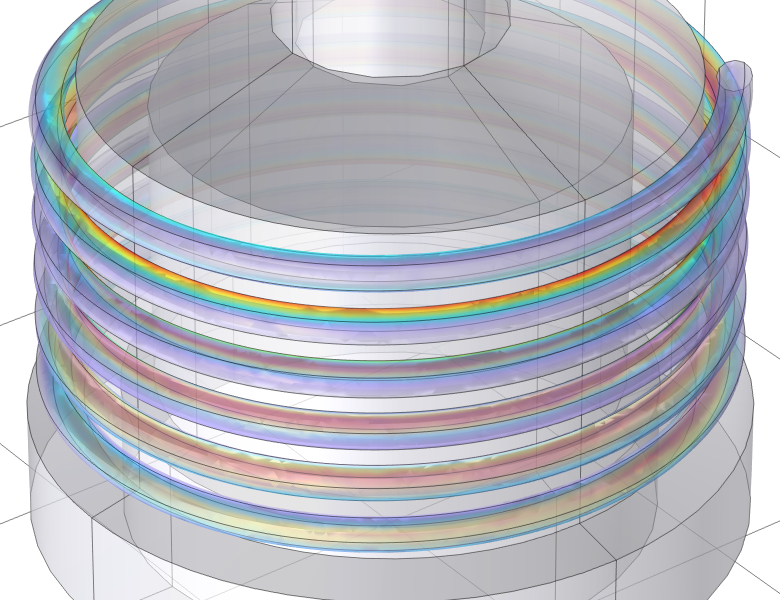
\includegraphics[width=\linewidth]{img/verlustdichte_closeup.png}
    \end{column}
  \end{columns}
  \vfill
\end{frame}

% ============================================================
\begin{frame}{Thermisches Ergebnis}
  \begin{columns}[T]
    \begin{column}{0.46\textwidth}
      \small
      \begin{tabular}{@{}L{1.6cm}L{1.9cm}L{1.9cm}@{}}
        \toprule
        \textbf{Körper} & \textbf{Min} & \textbf{Max} \\
        \midrule
        Spule & 257,7\,$^\circ$C & 335,6\,$^\circ$C \\
        Glas & 335,2\,$^\circ$C & 460,0\,$^\circ$C \\
        \bottomrule
      \end{tabular}

      \vspace{0.8em}
      Die Spule wird nicht von ihrem eigenen Strom heiß.\\
      Sie sieht durch den Millimeter Spalt fast nur glühendes Glas und nimmt dessen
      Strahlung auf.
    \end{column}
    \begin{column}{0.5\textwidth}
      \centering
      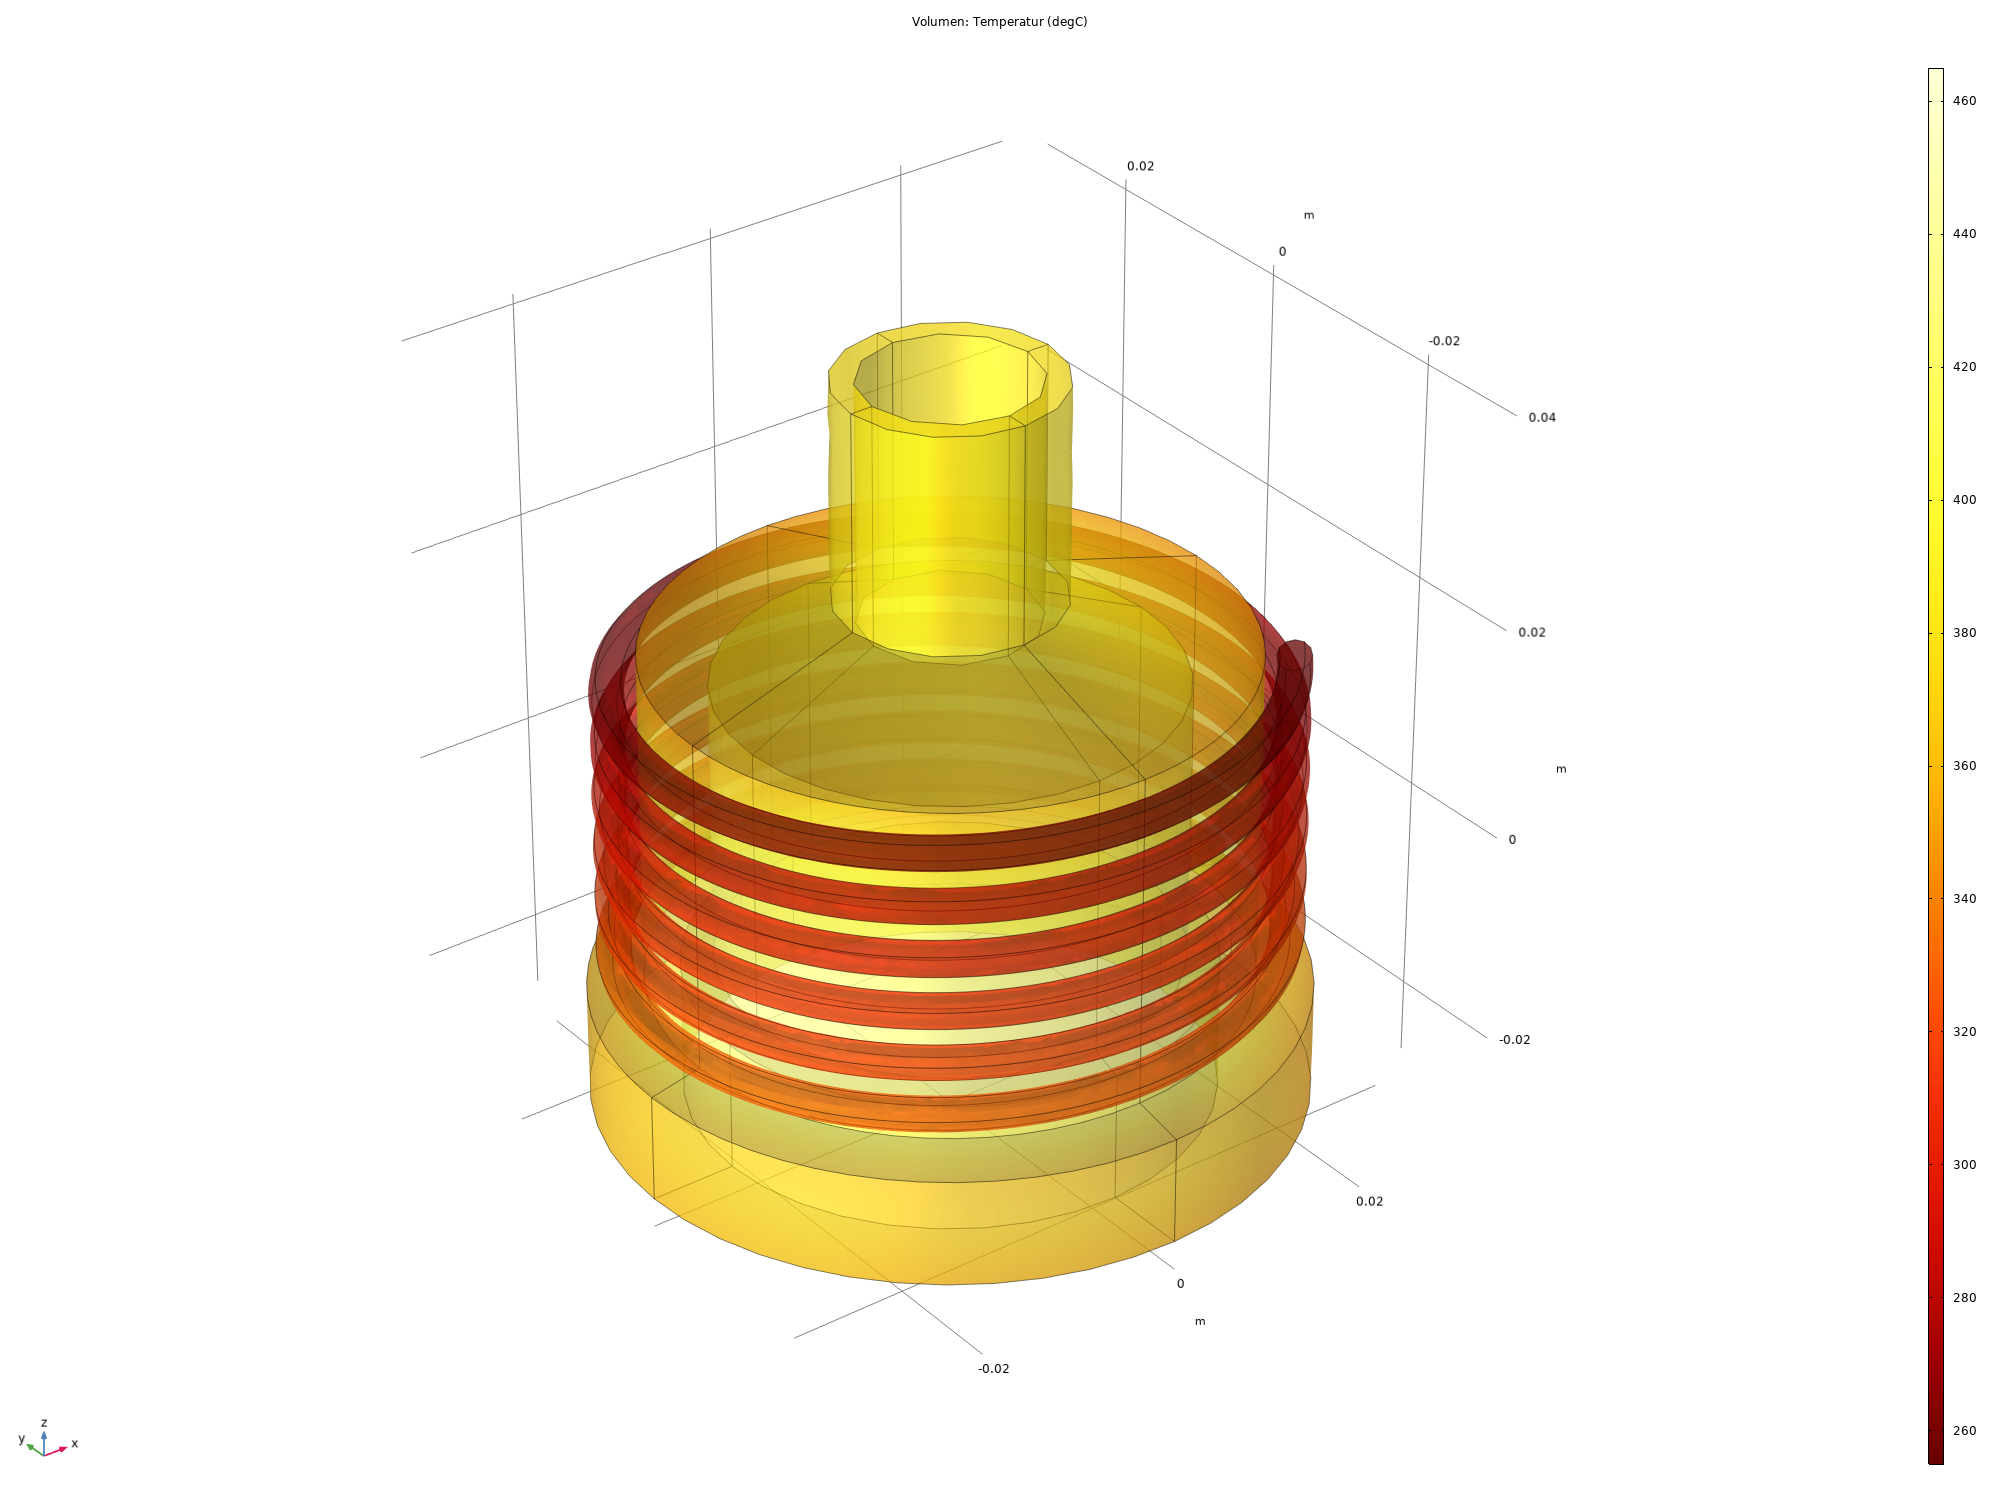
\includegraphics[width=\linewidth]{img/temperatur.png}
    \end{column}
  \end{columns}
\end{frame}

% ============================================================
\begin{frame}{Konsequenzen für die Hardware}
  \vfill
  \large
  \begin{itemize}
    \item Weichlot schmilzt bei 183 bis 190\,$^\circ$C, an der Spule muss hartgelötet oder geklemmt werden
    \item Viton-Dichtungen sind bei diesen Temperaturen erledigt, PTFE liegt an seiner Dauergrenze
    \item Kupfer verliert oberhalb von 200\,$^\circ$C seine Federhärte, die Wicklung braucht eine mechanische Halterung
    \item Das Quarzglas hat einen Erweichungspunkt von 1600\,$^\circ$C
  \end{itemize}
  \vfill
\end{frame}

% ============================================================
\begin{frame}{Validierung}
  \vfill
  \begin{itemize}
    \item Energiebilanz übers Strahlungsgleichgewicht: 545\,K erwartet, 531\,K simuliert
    \item Induktivität nach Wheeler: 4,6\,\% Abweichung
    \item Netz von 317.000 auf 441.000 Elemente verfeinert: Widerstand ändert sich um 4\,\%, Temperatur um 0,6\,\%
    \item Drei Läufe auf demselben Netz liefern identische Werte, auf ein Zehntel Milliwatt genau
  \end{itemize}
  \vfill
\end{frame}

% ============================================================
\begin{frame}{Nächste Schritte}
  \vfill
  \large
  \begin{itemize}
    \item Parameterstudie über die Plasmaleistung, 30 bis 100\,W
    \item Stromstudie von 3 bis 7\,A für die Generatorauslegung
    \item Temperaturabhängige Leitfähigkeit des Kupfers einbauen
  \end{itemize}
  \vfill
\end{frame}

% ============================================================
{
\setbeamertemplate{footline}{}
\begin{frame}[plain,c]
  \begin{tikzpicture}[remember picture, overlay]
    \node[anchor=north west, inner sep=0pt] at ([xshift=0.9cm,yshift=-0.6cm]current page.north west)
      {
\includegraphics[height=1.0cm]{img/JLU_Giessen-Logo.pdf}};
    \draw[giessenblau, line width=0.8pt] ([yshift=-1.7cm]current page.north west) -- ([yshift=-1.7cm]current page.north east);
    \draw[giessenblau, line width=0.8pt] ([yshift=1.6cm]current page.south west) -- ([yshift=1.6cm]current page.south east);
  \end{tikzpicture}
  \begin{center}
    {\LARGE\bfseries\color{giessenblau} Vielen Dank}\\[0.8em]
    {\Large\color{grauton} Fragen?}\\[2.2em]
    {\small\color{grauton} Konrad Wehkamp \quad\textperiodcentered\quad Koppeltest ABEP \quad\textperiodcentered\quad \vortragsdatum}
  \end{center}
\end{frame}
}

\end{document}
